\chapter{Richiami teorici}
\section{Teoria della similitudine}
L’applicazione della teoria della similitudine costituisce un primo e potente strumento della progettazione, in particolar modo per quanto riguarda le turbomacchine. La teoria della similitudine permette di risolvere diversi problemi:
\begin{itemize}
\item[$-$] note le prestazioni di una macchina che ha determinate dimensioni,
si possono ricavare le prestazioni di una macchina geometricamente simile a quella considerata ma di diverse dimensioni nel dettaglio permette la realizzazione di prototipi in scala ridotta (esempio tipico: modellino della grande turbina idraulica che viene provato prima di procedere alla costruzione della macchina vera);
\item[$-$] nota una ben determinata condizione di funzionamento di una turbomacchina, come potrebbero essere le condizioni di progetto, si possono individuare altre condizioni di funzionamento ottenute variando la velocità di rotazione, la portata, oppure il lavoro scambiato (fluido/macchina);
\item[$-$] curve di prestazioni rilevate in determinate condizioni ambientali possono essere espresse in funzione di parametri che sono invarianti al variare delle condizioni ambientali stesse. Possiamo conoscere le prestazioni di una macchina operante in condizioni diverse (ad esempio un compressore sul livello del mare ad agosto e in montagna a Natale);
\end{itemize}
Accanto a tutti questi aspetti riguardanti la capacità di predire le prestazioni di una macchina, si ritrova anche un ausilio al designer in sede di progettazione. Con la teoria della similitudine si può stabilire in maniera semplice e veloce fin da subito quale sarà il tipo di macchina migliore da usare, quale sarà la sua geometria di base e quali le dimensioni generali. Grazie a ciò si riesce a sfruttare l’esperienza già maturata nella progettazione, sviluppo e test di altre macchine simili. Possedere un database ricco di informazioni relative a macchine pregresse risulta essere un vantaggio progettuale non di poco conto.


ll teorema di Buckingham (conosciuto anche come teorema pi greco), dovuto al fisico statunitense Edgar Buckingham, afferma:
\begin{quoting}
Dato un problema descritto da un certo numero di equazioni in cui siano presenti $n$ variabili fisiche, se le dimensioni fondamentali di queste variabili sono $x$ allora il problema può essere completamente descritto da $n - x$ variabili adimensionali.
\end{quoting}
Per studiare il comportamento di una turbomacchina si definisce il seguente funzionale.
\begin{equation}
f(D_i,l_j,\dot{m},w,L_i,\mu,a_{01},\rho_{01})=0
\end{equation}
Con\\
$D_i$: serie di diametri rilevanti;\\
$l_j$: serie di lunghezze rilevanti;\\
$\dot{m}$: portata in massa;\\
$w$: velocità angolare;\\
$L_i$: lavoro ideale scambiato tra macchina e fluido per unità di massa;\\
$\mu$: viscosità dinamica del fluido;\\
$a_{01}$: velocità del suono all'ingresso in condizioni di ristagno;\\
$\rho_{01}$: densità del fluido.
\begin{equation}
Re= \frac{\rho_{01} w D^2}{\mu}
\end{equation}
\begin{equation}
Ma= \frac{w D}{a_{01}}
\end{equation}
Si evidenzia che tutti gli argomenti del funzionale sono descritti da una combinazione delle tre grandezze fondamentali M L T, ovvero massa lunghezza e tempo. Tenendo presente ciò è possibile adimensionalizzare gli argomenti del funzionale ottenendo una nuova espressione per lo stesso.

In una macchina termica in cui il fluido cambia le proprietà nei vari punti della macchina per definire la densità o la velocità del suono devo fissare
convenzionalmente una condizione rispetto alla quale vado a valutare quella
proprietà. 

Una condizione di riferimento che viene spesso adottata (non è
l’unica) potrebbe essere quella di valutare queste quantità nelle condizioni
totali all’ingresso della macchina (cioè condizioni valutate immaginando il fluido in quiete) che possiamo indicare con il pedice $01$ ($0$: condizioni totali o di ristagno; $1$: condizioni di ingresso).

Si può allo stesso modo definire le cifre di flusso $\Phi$ e di pressione $\psi$ andando ad adimensionalizzare rispettivamente la portata e il lavoro unitario:
\begin{equation}
\phi = \frac{\dot{m}}{w D^3}(=\frac{Q}{w D^3})
\end{equation}
\begin{equation}
\psi = \frac{L_i}{\rho_{01} w^2 D^2}
\end{equation}
Il funzionale può essere espresso quindi secondo i numeri adimensionali:
\begin{equation}
f(\pi_i,\pi_j,\phi,\psi,Re,Ma)=0
\end{equation}
Si può semplificare sotto le ipotesi di geometria simile.
\begin{equation}
f(\phi,\psi,Re,Ma)=0
\end{equation}
Supponendo di confrontare due macchine se queste hanno le gli stessi valori di $\pi_i$ e $\pi_j$, allora la geometria tra le due macchine sarà da considerarsi simile e sotto queste ipotesi il funzionale si semplifica come di seguito:
\begin{figure}
\centering
  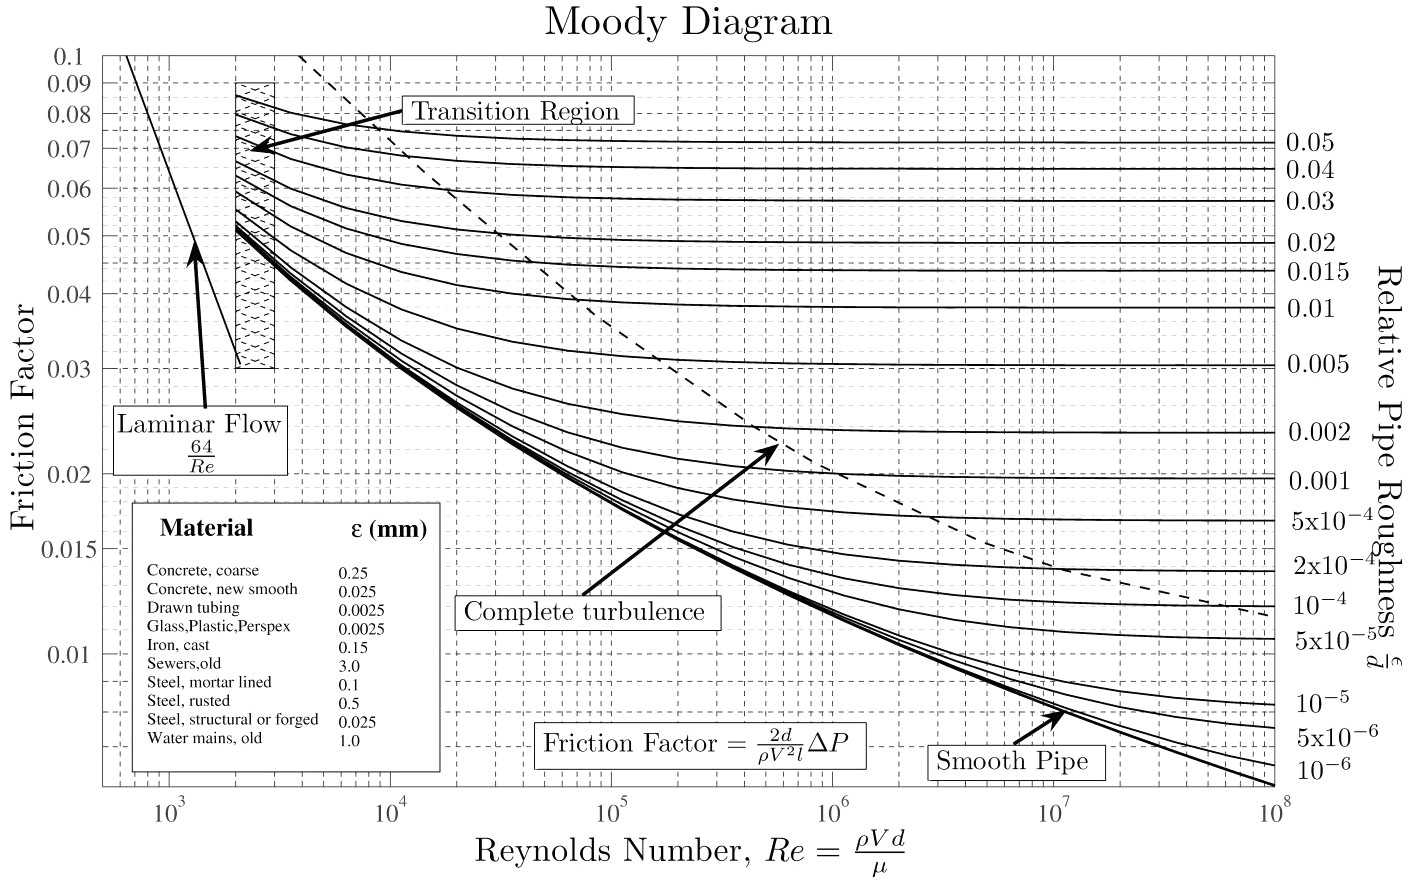
\includegraphics[width=\textwidth]{fig/moody.jpg}
\caption{}
\label{fig:moody}
\end{figure}
Guardando il diagramma di Moody in figura \ref{fig:moody}, in ascisse è presente $Re$ ed in ordinate il coefficiente di perdita di carico del nostro tubo $\xi$. Le scale sono logaritmiche. Il legame tra $\xi$ e $Re$, per bassi numeri di Reynolds, è rappresentato da una retta. Poi si ha una zona di transizione non ben definita ed infine una serie di linee a rugosità relativa costante $\epsilon/D$ (con $\epsilon$ rugosità media).

Nel primo tratto di legame lineare si ha una corrente laminare. Il tratto tratteggiato è un tratto nel quale, in condizioni sperimentali assolutamente controllate, è possibile mantenere un flusso laminare ma altamente instabile. In condizioni di flusso turbolento la perdita di carico dipende dalla rugosità.
Possiamo inoltre osservare che se consideriamo un solo valore di rugosità relativa la curva presenta una certa pendenza fino ad un certo valore di $Re$ (limite o critico) e poi diventa orizzontale. Sotto le ipotesi di moto turbolento pienamente sviluppato possiamo quindi trascurare l’influenza di Reynolds nel funzionale. Va ovviamente considerato che le rugosità relative di una macchina grande saranno in genere diverse da quelle che si possono ottenere con macchine piccole, quindi bisogna tenerlo presente. Variazioni anche grandi del numero di Reynolds, purché in regime di moto turbolento completamente sviluppato (corrispondenti a valori di Re molto elevati), non influenzano le prestazioni della mia macchina.

Se il numero di Reynolds è superiore ad un certo valore limite il coefficiente di perdita di carico è indipendente da $Re$. Se trasferiamo questa osservazione alla turbomacchina si può verificare sperimentalmente che se $Re$ è molto elevato questo potrà anche variare ma le prestazioni non ne saranno influenzate. Variazioni anche grandi del numero di Reynolds purchè siano nel
campo di $Re$ molto elevato, non influenzano le prestazioni della mia macchina.
\begin{equation}
f(\phi,\psi,Ma)=0
\end{equation}
In seguito, si aggiungerà una perdita sul modello in quanto il rendimento di una macchina piccola sarà sempre inferiore al rendimento di una macchina grande.

In ultimo se si considerano i fenomeni di comprimibilità trascurabili, si può trascurare anche il numero di Mach, equivalentemente si fa l'ipotesi $Ma\;<\;0.3$.
\begin{align*}
f(\Phi,\psi)=0
\end{align*}
Dotando la pompa di un sensore di pressione, giri e portata, posso andare a definire una curva di prestazione adimensionale.
Si definiscono orea le tre componenti del vettore velocità:
\begin{itemize}
\item[$c$]: velocità assoluta;
\item[$w$]: velocità relativa;
\item[$u$]: velocità periferica;
\end{itemize}
Naturalmente affinchè le macchine operino in condizioni di similitudine devono, per definizione, avere $\phi$ e $\psi$ uguali. 
\begin{equation}
\phi=\frac{Q}{w D^3} \propto \frac{c_m}{u}
\end{equation}

\begin{equation}
\psi = \frac{L_i}{w^2 D^2} \propto \frac{c_u}{u}
\end{equation}
Quindi, assegnato $D$, la cifra di flusso è proporzionale alla velocità meridiana e inversamente proporzionale a $u$ dove $u= \omega \times r$. La variazione di $c_u$ corrisponde alla variazione dell'energia cinetica a valle della macchina. 

Mantenere $\phi$ e $\psi$ uguali significa avere triangoli di velocità simili (vedi la figura \ref{fig:tria}).
\begin{figure}
\centering
  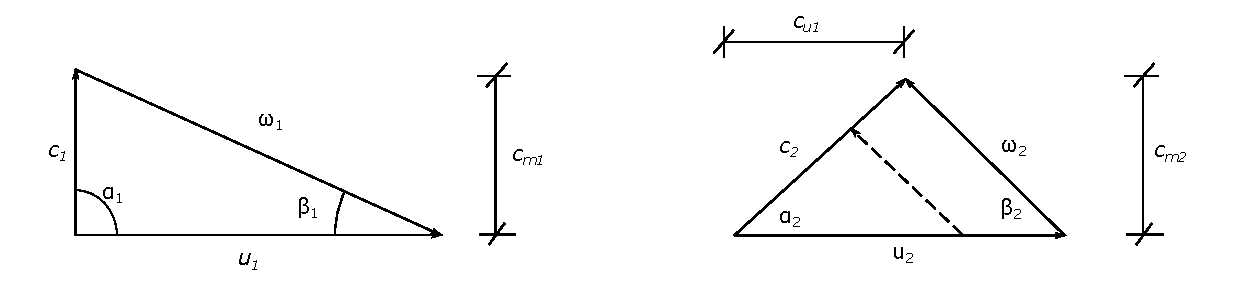
\includegraphics[width=.8\textwidth]{fig/triang.pdf}
\caption{}
\label{fig:tria}
\end{figure}
Consideriamo il caso di una macchina idraulica e vediamo come possiamo trovare il luogo dei punti di funzionamento simili sul piano delle prestazioni e quindi come le curve di prestazioni adimensionali stanno in rapporto con le curve di prestazioni dimensionali.

Se rileviamo le prestazioni di una pompa otteniamo la curva di funzionamento caratteristica (diagramma prevalenza-portata) per un certo valore della velocità di rotazione (figura \ref{fig:hq}).
\begin{figure}[h!]
\centering
  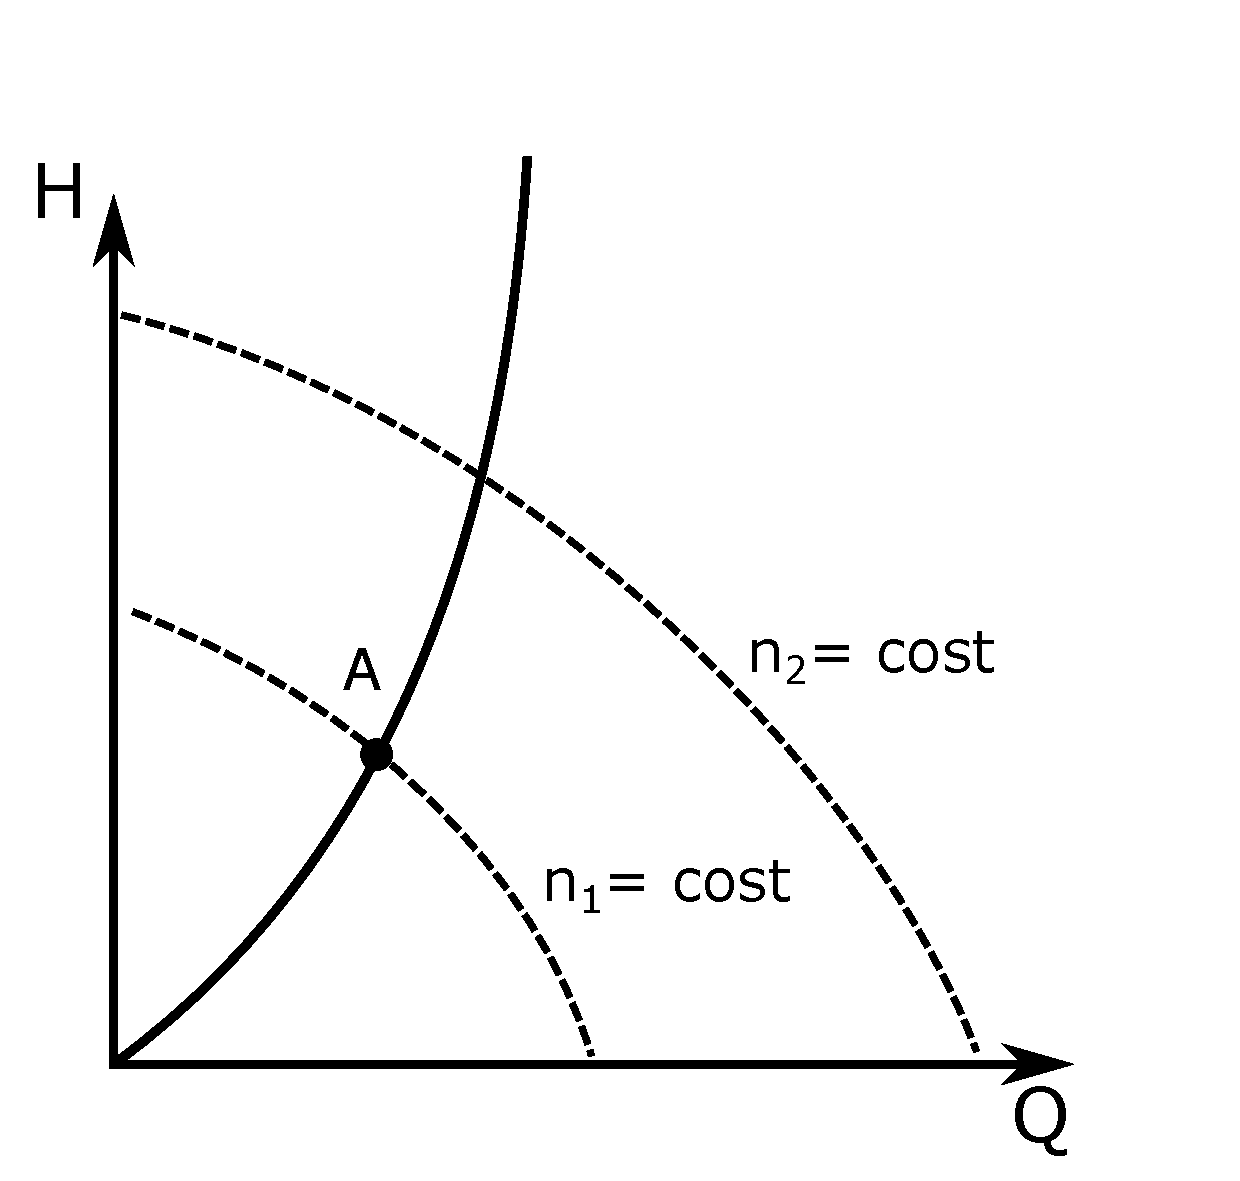
\includegraphics[width=.3\textwidth]{fig/hq.pdf}
\caption{}
\label{fig:hq}
\end{figure}
Queste sono curve espresse in funzione di grandezze dimensionali, ma andando ad adimensionalizzare si possono ottenere tali curve in funzione delle relative cifre di pressione e di flusso.  Si consideri un punto di funzionamento $A$, il luogo dei punti di funzionamento simili ad $A$ sarà caratterizzato dal fatto di avere stessi $\phi$ e $\psi$.

Considerando quindi il generico punto $x$ posso scrivere
\begin{equation}
\phi = \frac{Q}{w D^3}= \frac{Q_x}{w_x D^3}
\end{equation}
Considerando una macchina con lo stesso diametro posso scrivere
\begin{equation}
\frac{Q_x}{Q}=\frac{w_x}{w} \; \Rightarrow \; Q_x = Q \frac{w_x}{w}
\end{equation}
Imponendo invece l'uguaglianza della cifra di pressione
\begin{equation}
\psi = \frac{gH}{w^2 D^2}= \frac{gH_x}{w_x^2 D^2}
\end{equation}
In questo modo si ottiene
\begin{equation}
H_x = H(\frac{w_x}{w})^2 = H(\frac{Q_x}{Q})^2 \Rightarrow H_x = \frac{H}{Q^2}Q_x^2
\end{equation}
Che è l'equazione di una parabola sul piano H-Q, passante per il punto A e per l'origine degli assi. 
Noto che il lavoro varia al variare del quadrato della velocità angolare mentre la portata varia linearmente. 
Ad ogni curva $\phi - \psi$ corrisponde una curva di rendimento, posso quindi individuare una coppia $\bar{\phi} - \bar{\psi}$ ottimale (figura \ref{fig:adim}).
\begin{figure}[h!]
\centering
  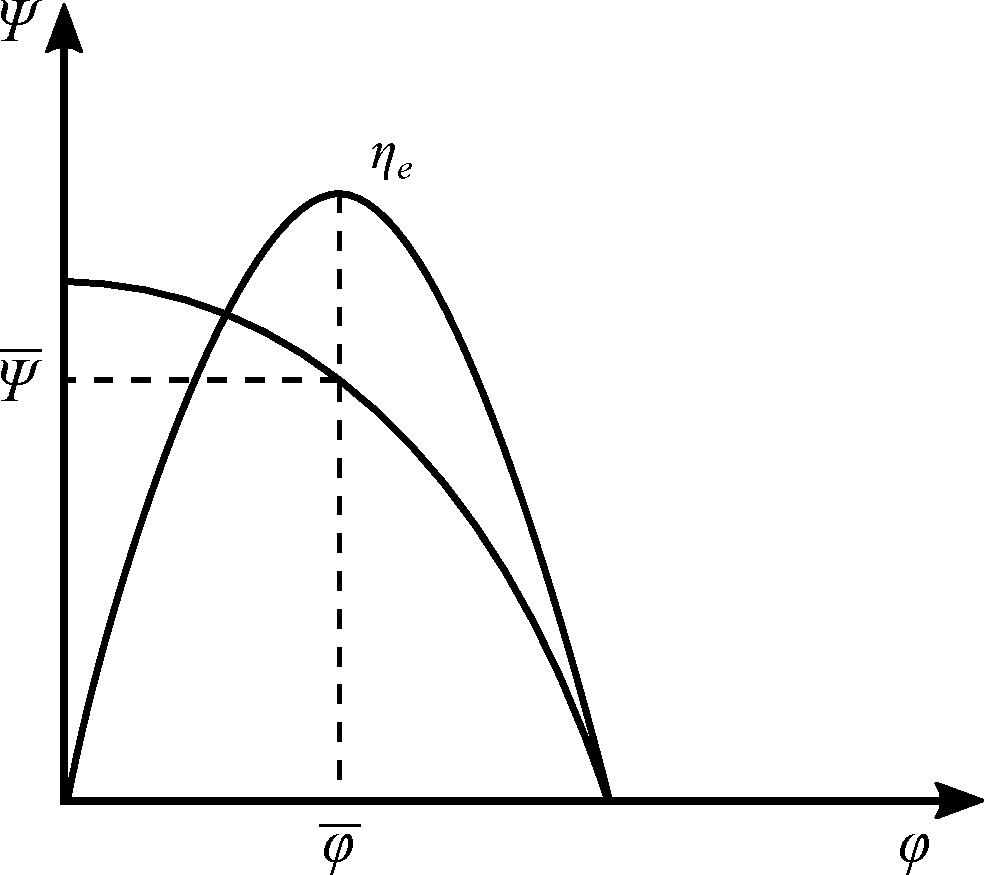
\includegraphics[width=.3\textwidth]{fig/adim.pdf}
\caption{}
\label{fig:adim}
\end{figure}
Posso anche definire il coefficiente di velocità periferica.
\begin{equation}
k_P = \frac{w D}{\sqrt{L_i}}
\end{equation}
Si tratta di una cifra che lega la velocità periferica della macchina al lavoro ideale della stessa.

Quando ho $\phi$ e $\psi$ posso definire una cifra di potenza adimensionalizzata come prodotto delle due.
\begin{equation}
\Lambda = \frac{P_e}{\rho w^3 D^5}
\end{equation}
Per macchina motrice
\begin{equation}
\Lambda = \phi \psi \eta_e
\end{equation}
Per macchina operatrice
\begin{equation}
\Lambda = \frac{\phi \psi}{\eta_e}
\end{equation}
Con la seguente espressione posso poi eliminare la caratteristica geometrica ottenere il numero specifico di macchina (o velocità specifica) che rappresenta una condizione di funzionamento lavoro-portata indipendente dalla dimensione della macchina. 
\begin{equation}
w_s = k = \phi^{1/2} \psi^{-3/4} = w \frac{\sqrt{Q}}{L_i^{3/4}}
\end{equation}
La forma della macchina varierà al variare di k . Avere dei k piccoli significa avere delle macchine nelle quali il termine di scambio di energia è prevalente rispetto al termine di portata. Questo numero permette, grazie all’esperienza storica (ovvero di tutti i dati che il progettista o la sua azienda possiedono in merito alle prestazioni di altre macchine), di classificare la forma geometrica di una macchina in base alle condizioni portata - lavoro.
\begin{figure}[h!]
\centering
  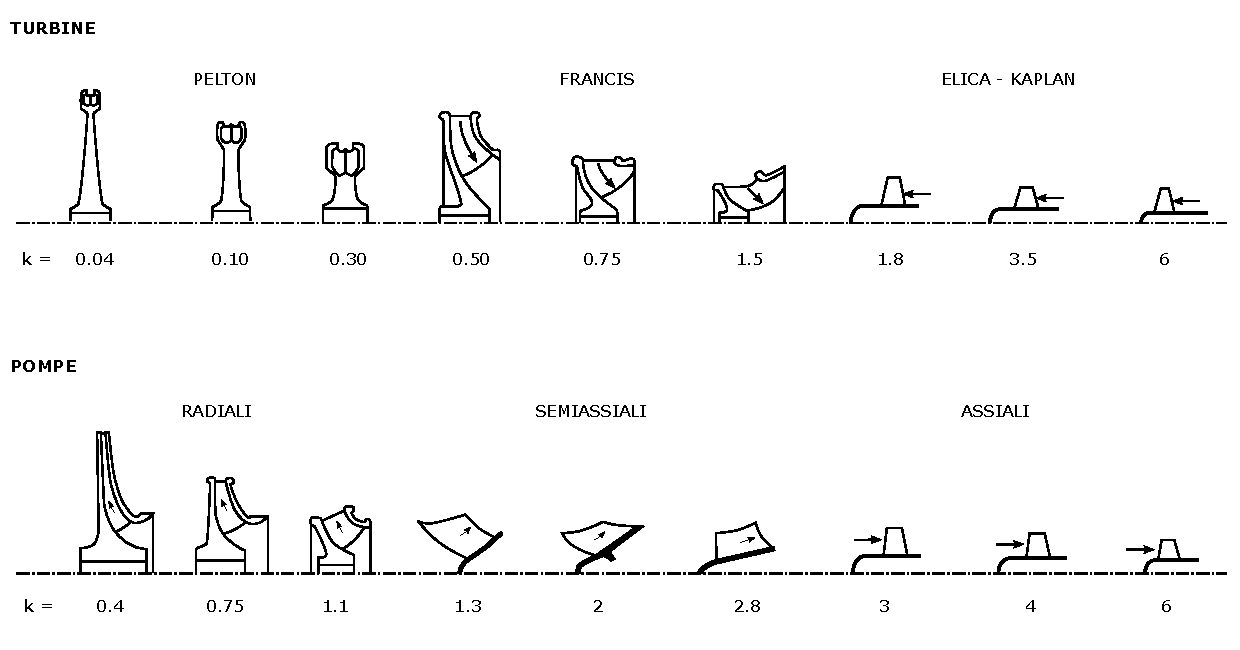
\includegraphics[width=\textwidth]{fig/numcar.pdf}
\caption{Variazione della forma delle giranti delle turbine idrauliche al variare del numero caratteristico di macchina.}
\label{fig:numcar}
\end{figure}
Queste cifre sono funzioni di k. Possono allora essere definite delle curve che riportano in ascissa il valore del numero caratteristico k e sulle ordinate i valori dei 4 rapporti.
Sfruttando l'esperienza possiamo analizzare le migliori macchine esistenti e vedere
quanto valgono per quelle macchine le cifre adimensionali $\pi_i$ , $\pi_j$ e diagrammarle in funzione di k . Facciamo un esempio concreto considerando una tipica macchina radiale (una pompa centrifuga) e consideriamo la sezione meridiana semplificata al massimo (figura \ref{fig:pala}).
\begin{figure}
\centering
\begin{minipage}{.5\textwidth}
  \centering
  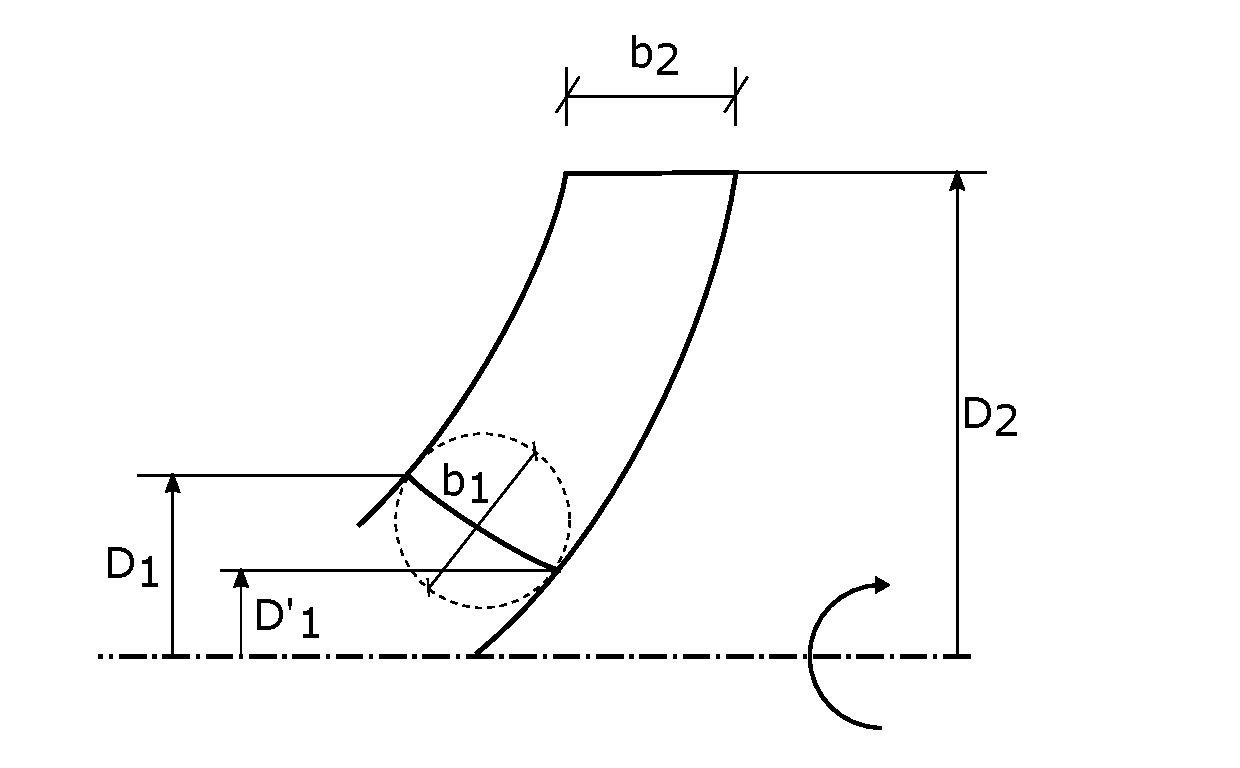
\includegraphics[width=.9\linewidth]{fig/pala.pdf}
  \captionof{figure}{}
  \label{fig:pala}
\end{minipage}%
\begin{minipage}{.5\textwidth}
  \centering
  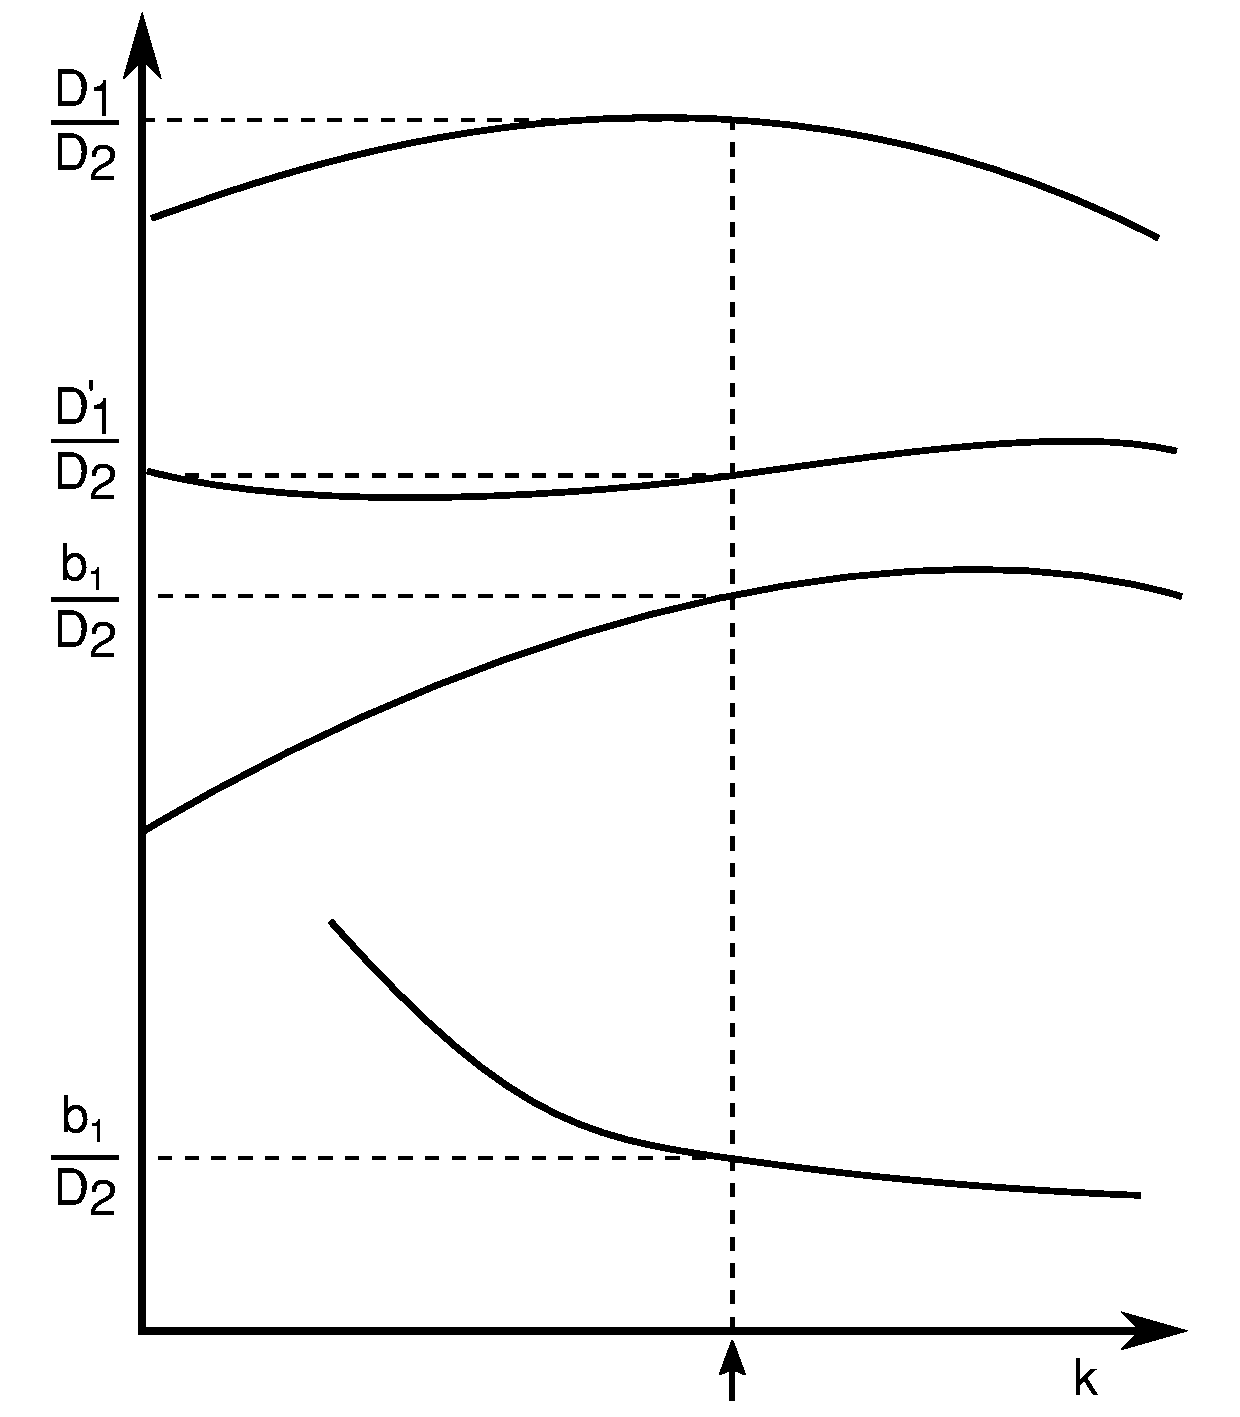
\includegraphics[width=.6\linewidth]{fig/primo_1.pdf}
  \captionof{figure}{}
  \label{fig:primo_1}
\end{minipage}
\end{figure}
Si definiscono le seguenti dimensioni caratteristiche più significative. Si tratta di un esempio didattico, in realtà posso andare a definire un database molto più ampio e raffinato. Siano
\begin{itemize}
\item[-]$D_2$: diametro massimo della girante;\\
\item[-]$D_1$: diametro massimo della sezione di ingresso;\\
\item[-]$D_1^{'}$: diametro minimo della sezione d'ingresso;\\
\item[-]$b_2$: altezza della pala in uscita;\\
\item[-]$b_1$: altezza della pala in ingresso.
\end{itemize}
Per definire $b_1$ bisogna prendere il diametro medio e con riferimento al punto di intersezione tra questo ed il profilo della pala in ingresso si traccia la circonferenza inscrivibile nella sezione d’ingresso. Come grandezza caratteristica della sezione d’ingresso prendo proprio il diametro di questa circonferenza.
Per queste grandezze posso definire le seguenti cifre adimensionali:
\begin{align*}
\frac{D_1}{D_2} \; \; \; \frac{D_1^{'}}{D_2} \; \; \; \frac{b_1}{D_2} \; \; \; \frac{b_2}{D_2} 
\end{align*}
Queste cifre sono funzioni di $k$. Posso allora essere definite delle curve che riportano in ascisse il valore del numero caratteristico $k$ ed in ordinate i valori dei 4 parametri.
Naturalmente fissato $k$ devo poi determinare il numero di giri a cui deve lavorare la macchina. 
Ricapitolando, note portata, prevalenza e fissata la velocità di rotazione, conosco il valore di $k$. Entrando in questi diagrammi si trovano i valori dei quattro parametri e quindi definisco per sommi capi la sezione meridiana della nostra macchina (figura \ref{fig:primo_1}).

Esiste una dimensione ottimale cioè una dimensione alla quale corrisponde il massimo rendimento. Bisogna però definire un’ulteriore grandezza detta diametro specifico.
\begin{equation}
D_s= \phi^{-1/2} \psi^{1/4} = D \cdot \frac{L_i^{1/4}}{\sqrt{Q}}
\end{equation}
Bisogna cercare di eliminare la velocità di rotazione. È stato verificato che esiste, con riferimento alle dimensioni di massimo rendimento, un legame tra $D_s$ e $w_s$. 
\begin{equation}
D_s=f(w_s)
\end{equation}
Questa funzione è descritta empiricamente sul \textit{Diagramma di Cordier}. Questo diagramma rappresenta l’interpolazione di una serie di dati sperimentali (da vedere come correlazione statistica).
Grazie alle curve di Balié è possibile osservare l’entità delle variazioni che si ottengono andando a discostarsi, entro certi limiti, dalla curva di Cordier.
Si può estendere questa relazione con i diagrammi di Baliè, intorno alla curva si disegnano curve di isorendimento.
\begin{figure}
\centering
\begin{minipage}{.5\textwidth}
  \centering
  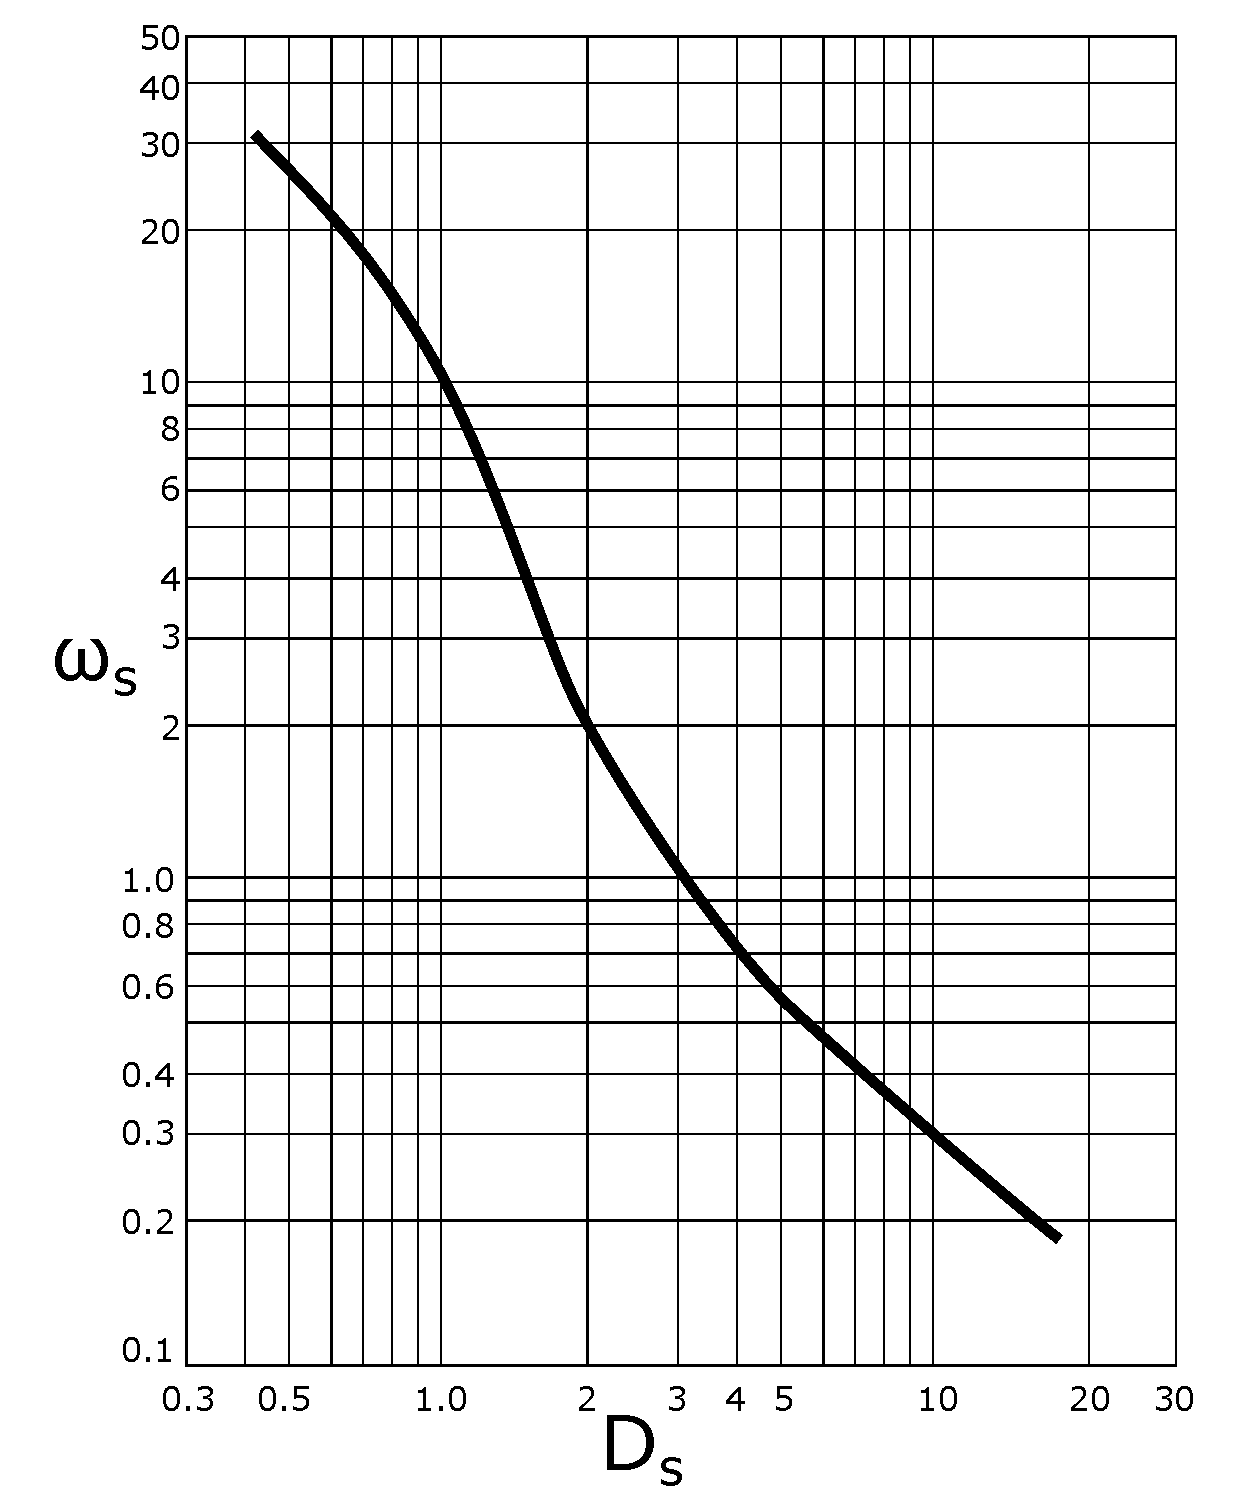
\includegraphics[width=.95\linewidth]{fig/cord_diag.pdf}
  \captionof{figure}{Diagramma di Cordier}
  \label{fig:cord_diag}
\end{minipage}%
\begin{minipage}{.5\textwidth}
  \centering
  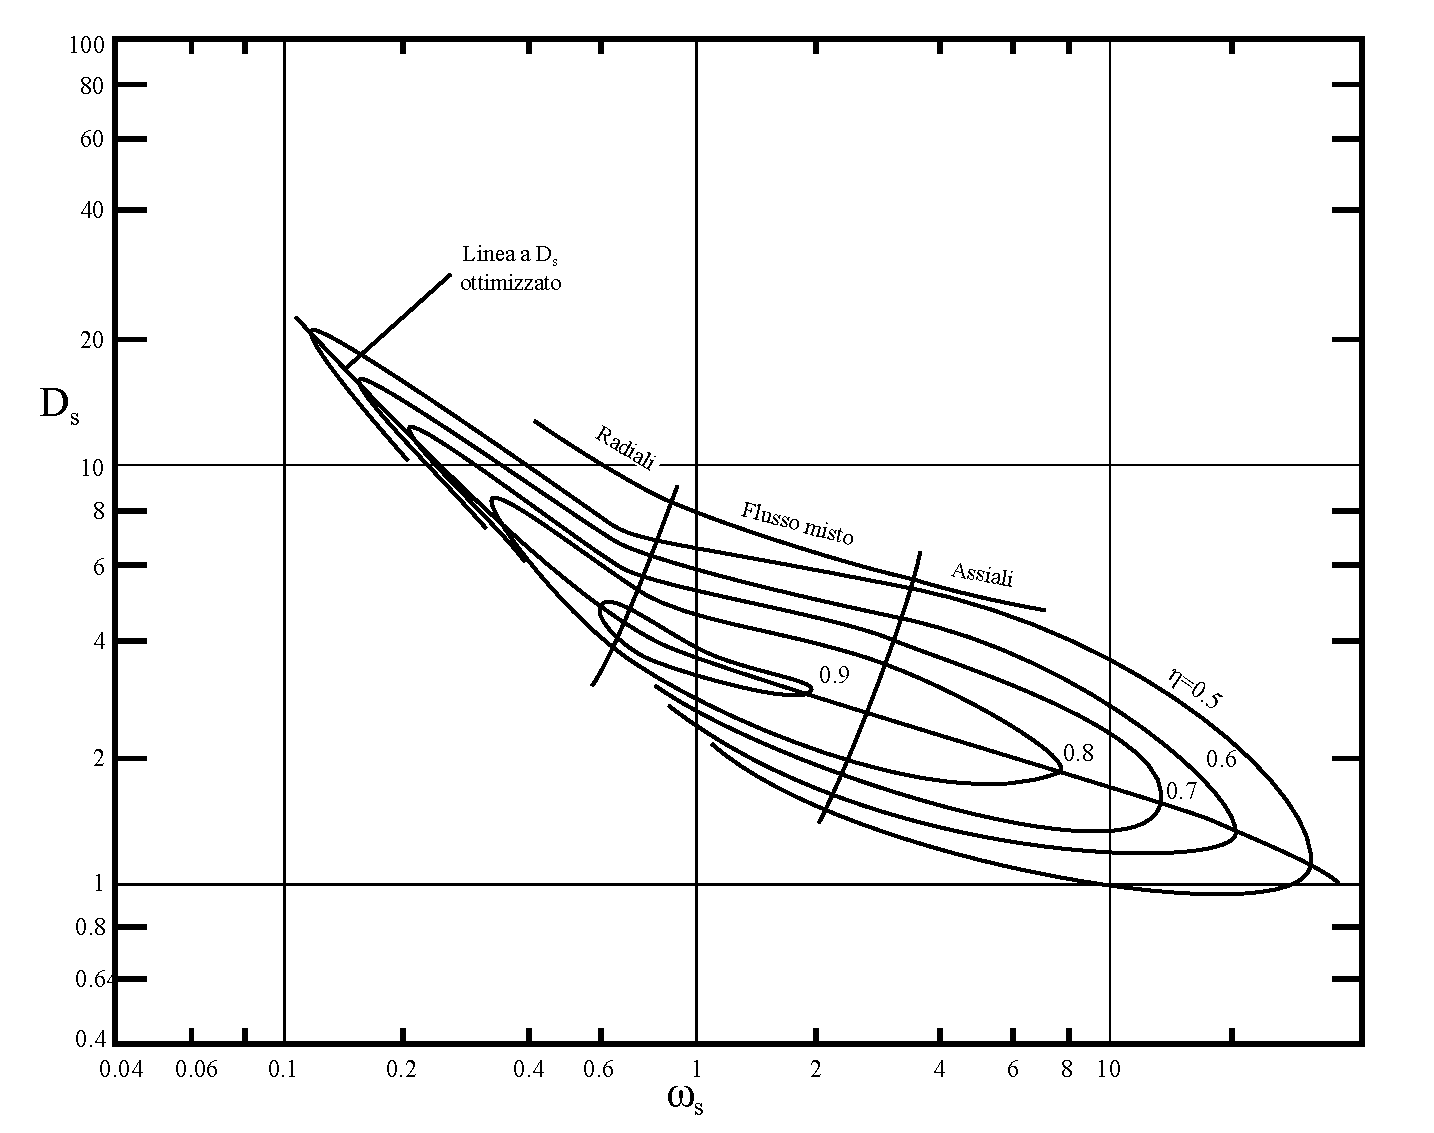
\includegraphics[width=.95\linewidth]{fig/primo_3.pdf}
  \captionof{figure}{}
  \label{fig:primo_3}
\end{minipage}
\end{figure}

\section{Influenza di Re}
Queste considerazioni sono state fatte trascurando l'influenza di Re. Ricordando il diagramma di Moody la relazione è fatta rispetto a $\epsilon/D$. Per le macchine è essenzialmente uguale, al diminuire di Re le curve si spostano più in basso, questo effetto si riflette in un abbassamento di rendimento e quindi di prevalenza.

Questo è un fenomeno prevedibile in termini statistici, storicamente grazie all'accumulazione di dati sono stati definiti due fattori di correzione, di rendimento $f_\eta$ e $f_\psi$ diagrammati ripsetto a $Re$. Man mano che $Re$ scende il loro effetto diventa sempre più importante. 
\begin{figure}
\centering
\begin{minipage}{.4\textwidth}
  \centering
  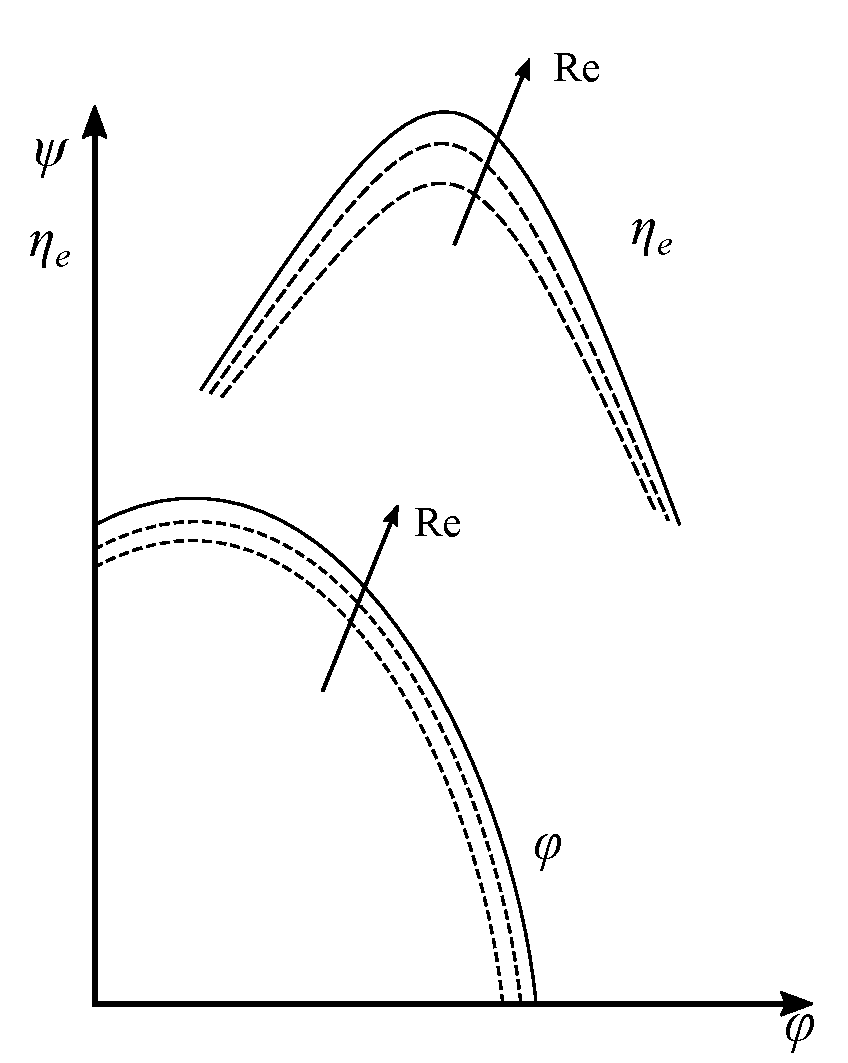
\includegraphics[width=.95\linewidth]{fig/secondo_1.pdf}
  \captionof{figure}{}
  \label{fig:secondo_1}
\end{minipage}%
\begin{minipage}{.6\textwidth}
  \centering
  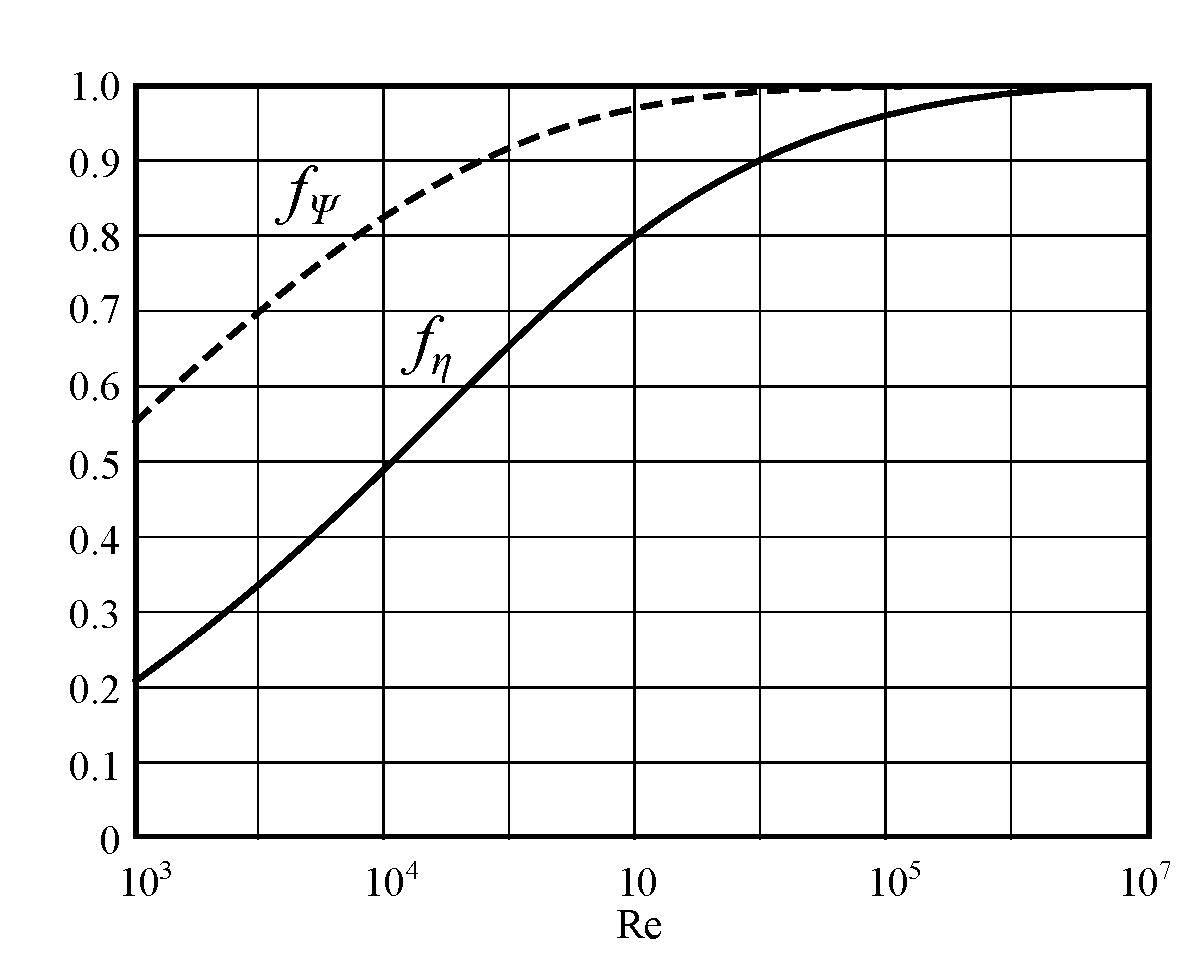
\includegraphics[width=.95\linewidth]{fig/secondo_2.pdf}
  \captionof{figure}{}
  \label{fig:secondo_2}
\end{minipage}
\end{figure}

Parto dalla $w_s$, scrivo $\Phi$ e $\psi$ nei diversi punti di funzionamento della macchina in funzione di $w_s$ ($\equiv k$). 
\begin{align*}
w_s= \phi^{1/2}\psi^{-3/4} \Rightarrow 
\begin{cases}
\psi = \psi(w_s)\\
\eta = \eta(w_s)
\end{cases}
\Rightarrow
\begin{cases}
f_{\psi} = f(Re)\\
f_{\eta} = f(Re)
\end{cases}
\end{align*}
Con i coefficienti correttivi vado a trovare le cifre adimensionali corrette \begin{align*}
\begin{cases}
\psi_{corretto} = f_{\psi} \cdot \psi(w_s)\\
\eta_{corretto} = f_{\eta} \cdot \eta(w_s)
\end{cases}
\end{align*}
A questo punto è possibile procedere a ritroso. Trovato il valore corretto avrò
\begin{align*}
\omega_s = \phi^{1/2} \psi^{-3/4} =  \phi_{corretto}^{1/2} \psi_{corretto}^{-3/4} = cost
\end{align*}
partendo proprio dalla definizione di $\omega_s$ è possibile costruire le curve di prestazione corrette.

\section{Effetto scala}
Si considera poi un effetto scala non solo legato alle rugosità superficiali ma anche legato ai giochi. L'effetto scala può essere espresso rispetto ai rapporti dimensionali. Queste relazioni sono sempre costruite per via empirica sulla base dei dati storici.

A parità di bontà di progettazione, geometria, ecc... la macchina grande ha un rendimento maggiore rispetto alla macchina piccola. Questo si spega facendo due osservazioni: a parità di tecnologia produttiva è possibile ritenere costante il valore della rugosità superficiale delle palettature della girante. In una macchina grande la rugosità relativa sarà quindi più bassa, quindi le perdite di carico saranno superiori nella macchina piccola. In secondo luogo bisogna tener conto dei giochi presenti tra parte fissa e parte mobile, che non possono scendere al di sotto di un certo limite. Nelle macchine grandi questi diventeranno trascurabili. 
\begin{figure}
\centering
  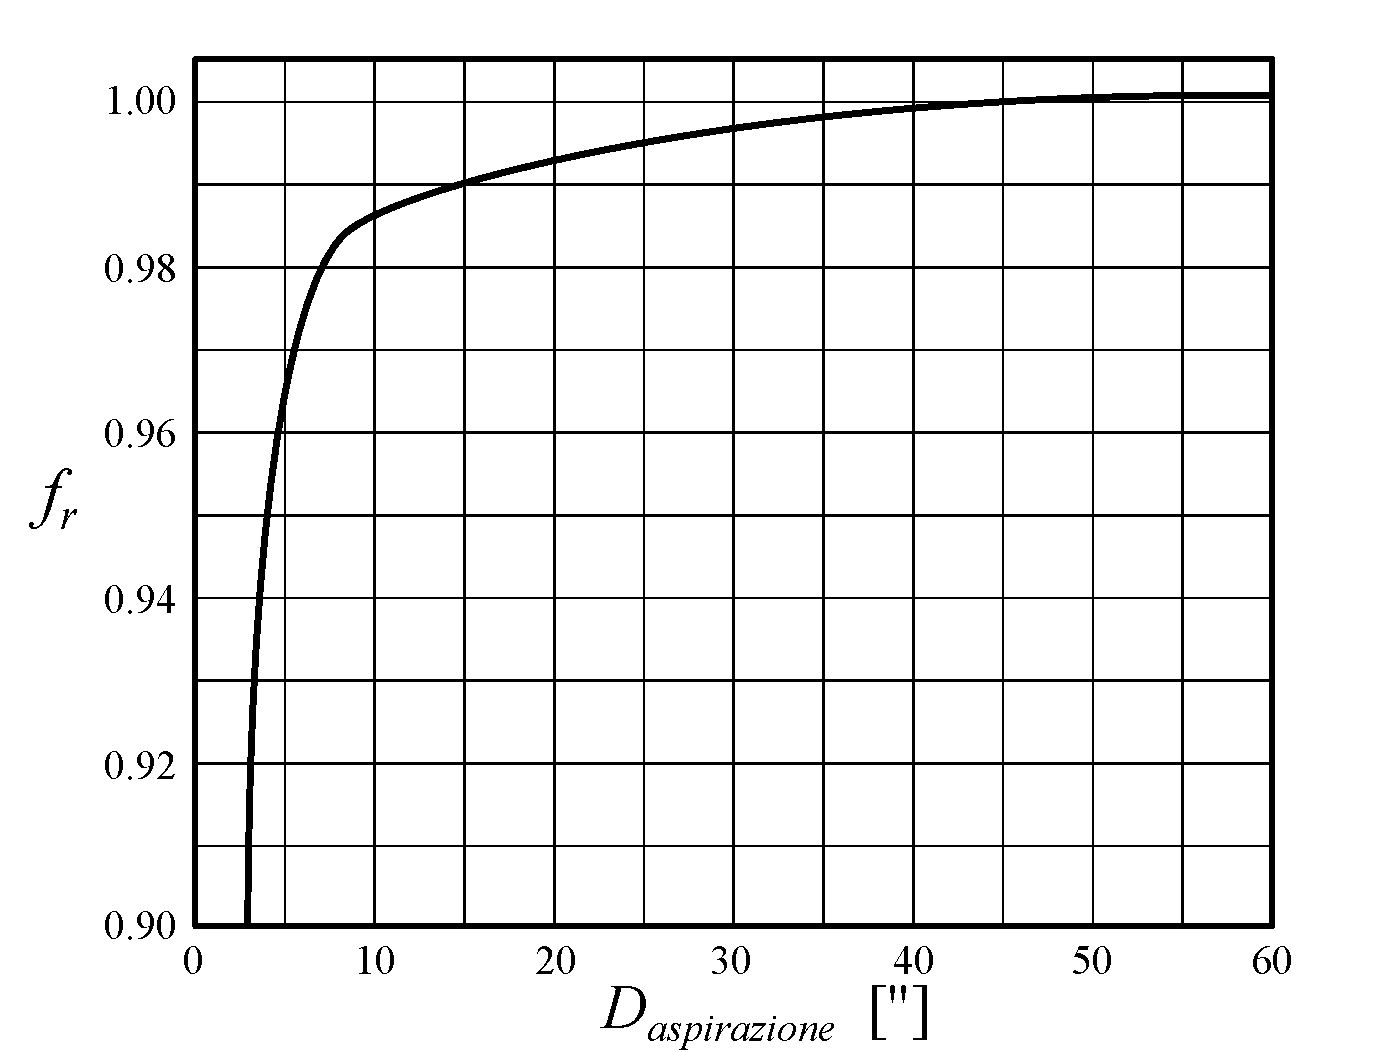
\includegraphics[width=.5\textwidth]{fig/dDchart.pdf}
\caption{}
\label{fig:dDchart}
\end{figure}

Facendo riferimento alle pompe possiamo definire un rapporto dimensionale 
\begin{align*}
\frac{D_1}{D_2} \triangleq  \mbox{Rapporto di scala}, \; D_1 < D_2
\end{align*}
In riferimento alla figura \ref{fig:dDchart} rendimento si può esprimere come
\begin{align*}
\eta = \eta_S \cdot f_r(D)
\end{align*}
E la relazione tra il rendimento tra le pompe di scala diversa è il seguente
\begin{equation}
\frac{1-\eta_1}{1-\eta_2} = \left( \frac{D_2}{D_1}\right)^\alpha
\end{equation}
La stessa operazione viene fatta per le turbine idrauliche
\begin{align*}
\frac{1-\eta_1}{1-\eta_2} = \left[ \frac{Re_{u,2}}{Re_{u,1}} \right]^n, \; \; n=0.1 \div 0.25
\end{align*}
\begin{align*}
\frac{1-\eta_1}{1-\eta_2} =0.5 + 0.5 \left[ \frac{Re_{u,2}}{Re_{u,1}} \right]^{0.2}
\end{align*}
\begin{align*}
\frac{1-\eta_1}{1-\eta_2} = 0.3 + 0.7 \left[ \frac{Re_{u,2}}{Re_{u,1}} \right]^{0.2} \; \to \; \mbox{Turbine Kaplan}
\end{align*}
\section{Flusso comprimibile}
Se si considera il flusso comprimibile le relazioni diventano più complesse. Infatti si ha:
\begin{equation}
\psi=f(\phi,Ma)
\end{equation}
$\psi$ dipende quindi anche dal numero di Mach. 
Nel diagramma $\phi-\psi$ si ottengono diverse curve al variare del numero di Mach (Figura \ref{fig:ComprMach}), le curve diventano poco leggibili. Posso infatti ottenere lo stesso valore di lavoro giocando sulle grandezze di T-p, non ho più una definizione univoca di lavoro. Si tratta di una rappresentazione poco fisica e di un esercizio esclusivamente accademico.
\begin{figure}[h!]
\centering
  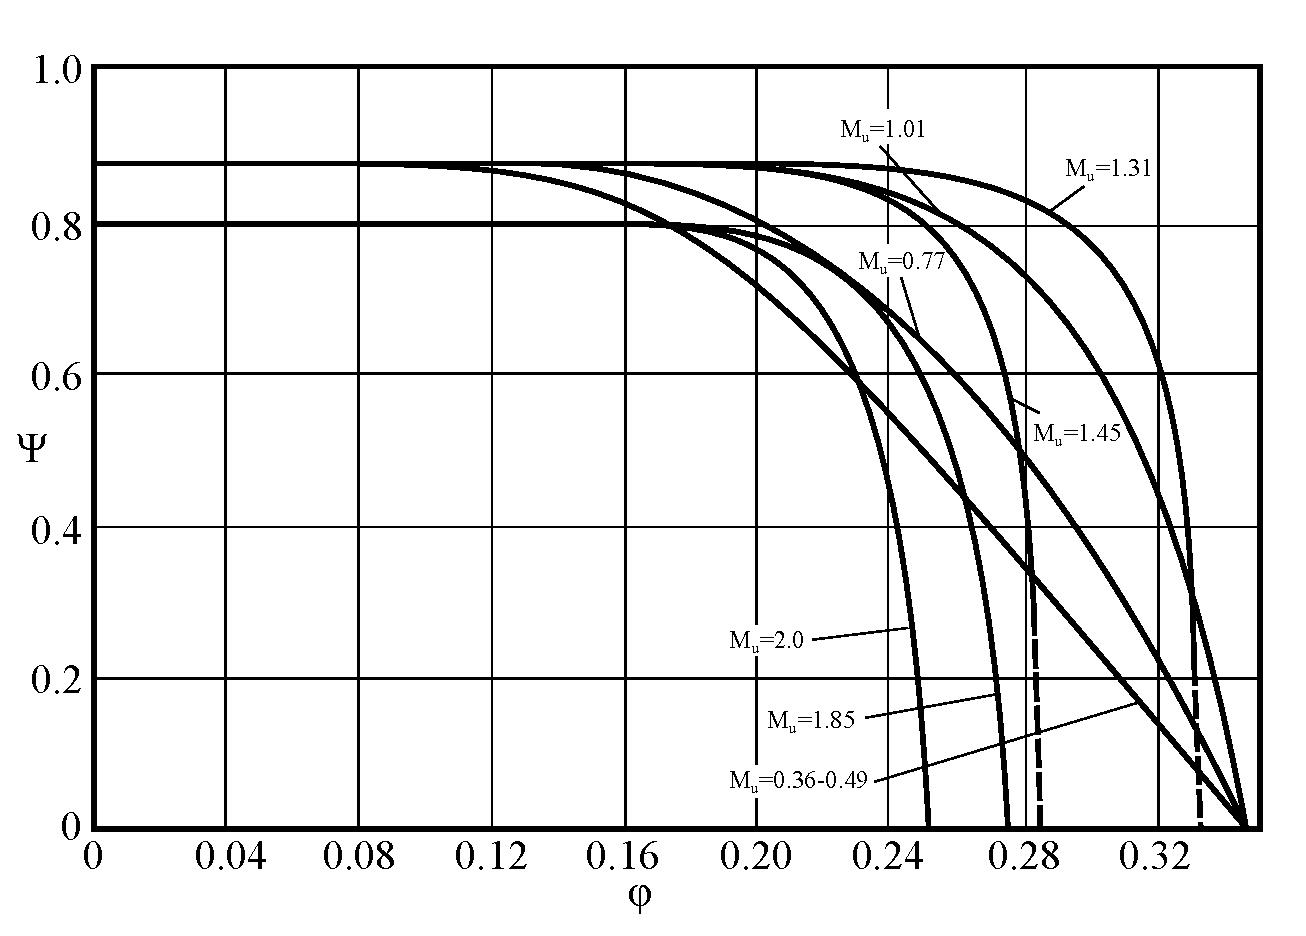
\includegraphics[width=.85\textwidth]{fig/ComprMach.pdf}
\caption{Curve adimensionali di funzionamento di una famiglia di compressori, per un fluido assegnato, a diversi numeri di Mach periferici. Sono definiti $Ma = \frac{w \frac{D}{2}}{a_{01}}$, $Mu = \frac{w \frac{D}{2}}{a}$}
\label{fig:ComprMach}
\end{figure}
Per questo tipo di macchine si utilizzaranno curve molto diverse. Per avere una grandezza confrontabile di funzionamento devo rendere qualsiasi prova io faccia a grandezza standard. In questo modo posso rappresentare condizioni di funzionamento in modo univoco. 
Definisco il significato dei pedici:
\begin{itemize}
\item $s$: grandezze relative alle condizioni standard;
\item $c$: valori corretti, cioè riportati alle condizioni standard;
\item "  ": valori da correggere rilevati nel corso della prova.
\end{itemize}
Proprietà di un gas generico miscela di due gas con massa molare M:
\begin{equation}
\frac{p}{\rho} = \frac{p_1}{\rho} + \frac{p_2}{\rho} = x_1  \frac{p_1}{\rho_1} + \frac{p_2}{\rho_2} = RT \left( \frac{x_1}{M_1} + \frac{x_2}{M_2} \right) = RT(\frac{1}{M})
\end{equation}
\begin{equation}
c_P = x_1 c_{P1} + x_2 c_{P2}
\end{equation}
\begin{equation}
\cfrac{\gamma}{\gamma -1} = \cfrac{\frac{x_1}{M_1} \cfrac{\gamma_1}{\gamma_1 -1}+\cfrac{x_2}{M_2} \cfrac{\gamma_2}{\gamma_2 -1}}{\cfrac{x_1}{M_1}+\cfrac{x_2}{M_2}}
\end{equation}
Rapporto di compressione standard:
\begin{equation}
\frac{p_{02}}{p_{01}} = \frac{p_{01c}}{p_{01s}} \; \Rightarrow \; p_{02c} = p_{02}\frac{p_{01s}}{p_{01}}
\end{equation}
Parametro di portata
\begin{equation}
\frac{\dot{m}\sqrt{T_{01}}}{p_{01}}=\frac{\dot{m_c}\sqrt{T_{01s}}}{p_{01s}} \; \Rightarrow \; \dot{m_c} = \dot{m} \sqrt{\frac{T_{01}}{T_{01s}}} \bigg(\frac{p_{01s}}{p_{01}} \bigg)
\end{equation}
Parametro di velocità
\begin{equation}
\frac{n}{\sqrt{T_{01}}}=\frac{n_c}{\sqrt{T_{01s}}} \; \Rightarrow \; n_c = n \sqrt{\frac{T_{01s}}{T_{01}}}
\end{equation}
Si definiscono quindi le condizioni ambientali standard.
\begin{multicols}{2}
Pressione ridotta
\begin{equation}
\delta = \frac{p_{01}}{p_{01s}}
\end{equation}
Temperatura ridotta
\begin{equation}
\theta = \frac{T_{01}}{T_{01s}}
\end{equation}
\end{multicols}
Si ottiene:
\begin{align*}
p_{01c} = \frac{p_{02}}{\delta}
\end{align*}
\begin{align*}
\dot{m_c}= \dot{m} \frac{\sqrt{\theta}}{\delta}
\end{align*}
\begin{align*}
n_c = \frac{n}{\sqrt{\theta}}
\end{align*}
\begin{figure}
\centering
  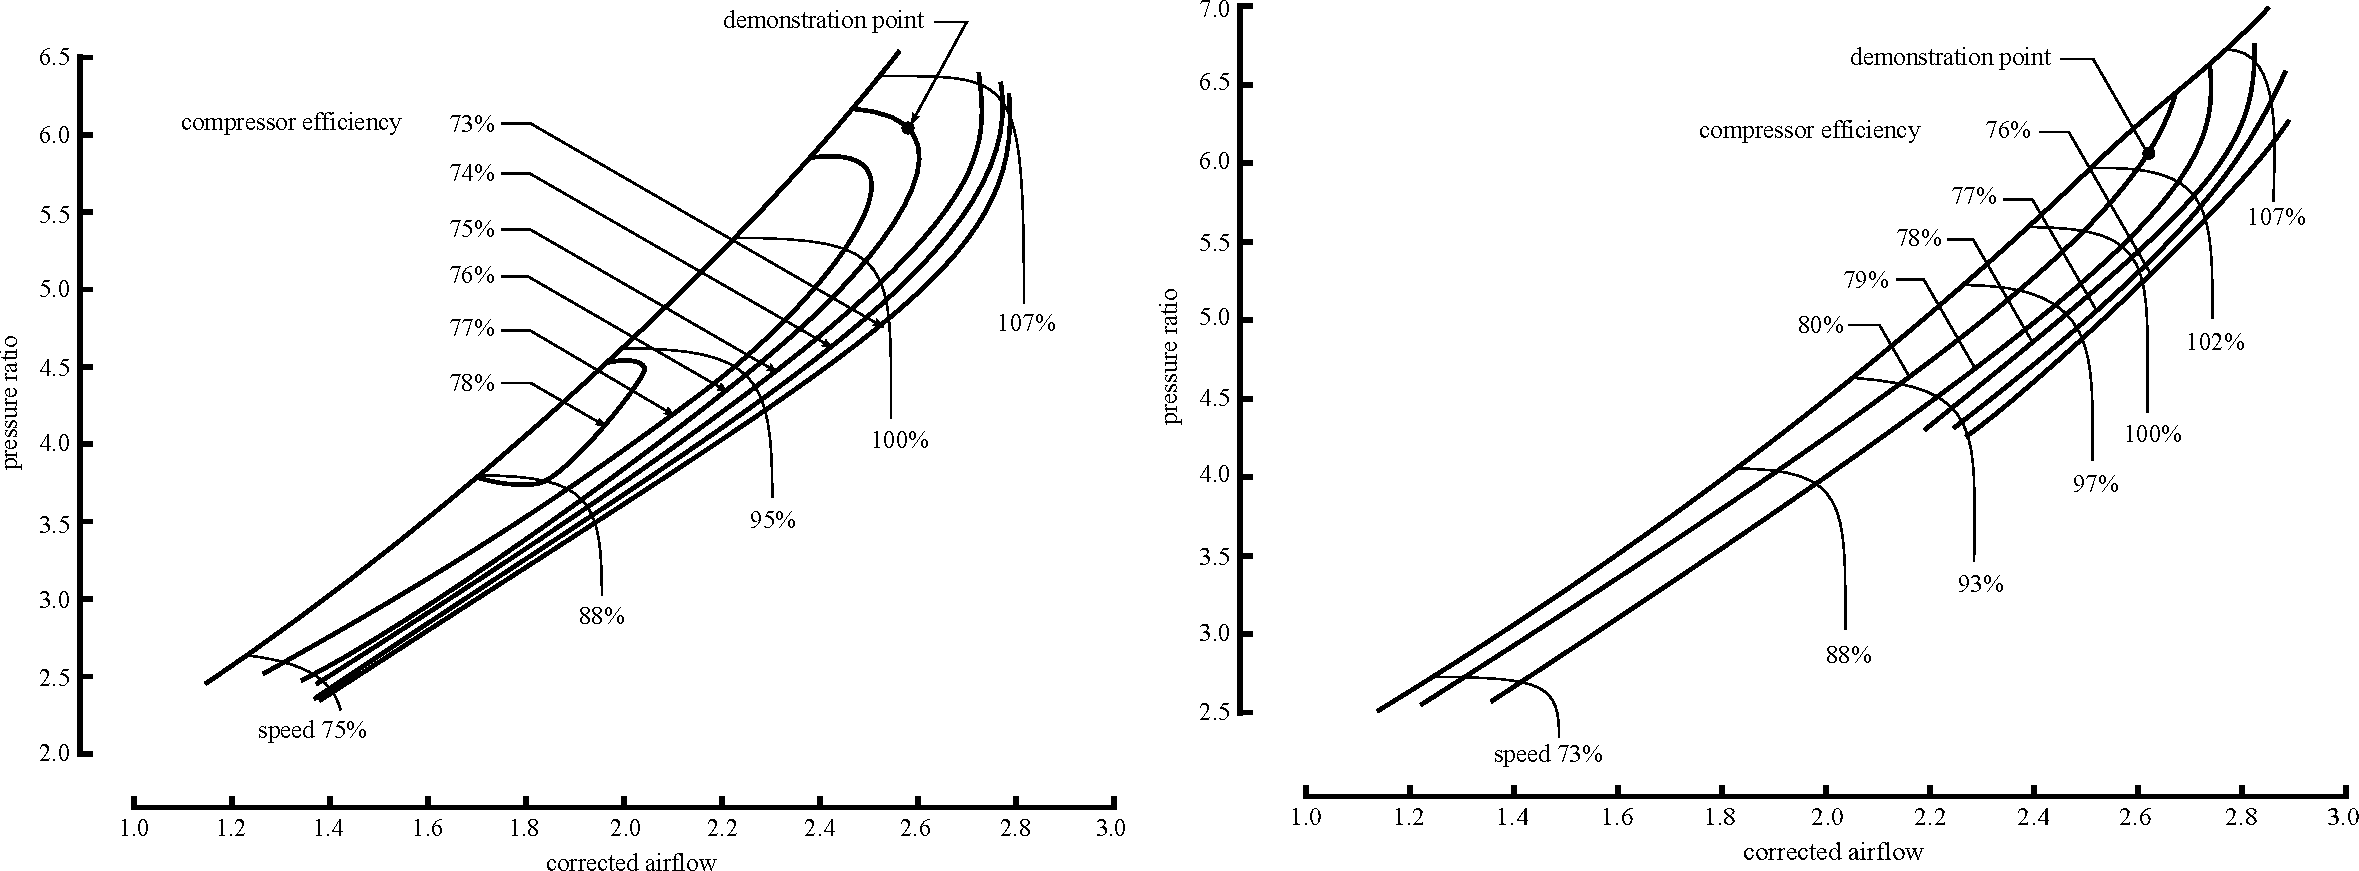
\includegraphics[width=\textwidth]{fig/CompMaps.pdf}
\caption{}
\label{}
\end{figure}
Si ottiene così la portata di massa corretta e il numero di giri corretto.
In questo modo si trovano le mappe di funzionamento delle macchine. Si diagrammano la portata d'aria corretta con il rapporto di compressione. Sono tracciate diverse curve al variare dei giri con le curve di isorendimento.

A questo punto si espande l'espressione di $\phi$.
\begin{align*}
M_{01}=\frac{w D}{a_{01}}= \frac{w D}{\sqrt{k R T_{01}}}, \;\;\;p = \rho_i RT, \;\;\; a = \sqrt{k R T}
\end{align*}
\begin{equation}
\phi = \frac{\dot{m}}{\rho_{01} w D^3} = \frac{\dot{m}}{\rho_{01} M_{01} a_{01} D^2} = \frac{\dot{m} R T_{01}}{\rho_{01} M_{01} \sqrt{k R T_{01}} D^2} = \frac{\dot{m} \sqrt{R T_{01}}}{\rho_{01} M_{01} \sqrt{k} D^2}
\end{equation}
\begin{equation}
\psi = \cfrac{L_i}{w^2 D^2} = \cfrac{\Delta h_{0s}}{w^ 2 D^2} = \cfrac{\cfrac{k}{k-1} R T_{01}\left[ \bigg( \cfrac{p_{02}}{p_01} \bigg)^{\frac{k-1}{k}}-1\right]}{M_{01}^2 k R T_{01}} = \cfrac{\cfrac{1}{k-1} \left[ \bigg( \cfrac{p_{02}}{p_01} \bigg)^{\frac{k-1}{k}}-1\right]}{M_{01}^2 }
\end{equation}

L'idea è quella di rappresentare in modo univoco il comportamento del compressore usando i termini $\phi$, $\psi$ ma mantenendo la significatività fisica.

Se utilizzo lo stesso fluido posso trascurare $R$ e $k$. Utilizzando la stessa macchina trascuro anche $D$, riferendosi alle condizioni standard posso considerare $M_{01}=cost$. Ricavo le seguenti relazioni semplificate:
\begin{align*}
M_{01} \to \frac{w D}{\sqrt{R T_{01}}} \Rightarrow M_{01} \to \frac{w}{\sqrt{T_{01}}}
\end{align*}
\begin{align*}
\phi \to \frac{\dot{m} \sqrt{RT_{01}}}{\rho_{01} D^2} \Rightarrow \phi \to \frac{\dot{m} \sqrt{T_{01}}}{\rho_{01}}
\end{align*}
\begin{align*}
\psi \to \frac{p_{02}}{p_{01}}
\end{align*}
Si tratta di grandezze che posso andare a misurare in un banco prova. 
La mappa di funzionamento del compressore assume quindi una forma più leggibile, sull'asse delle ascisse ho la portata in massa corretta con la temperatura in ingresso e sulle ordinate il rapporto di compressione. Assieme a queste posso anche costruire le linee di isorendimento  e quindi la curva ideale operativa del compressore data dall'inviluppo delle curve di isorendimento.
\begin{figure}
\centering
  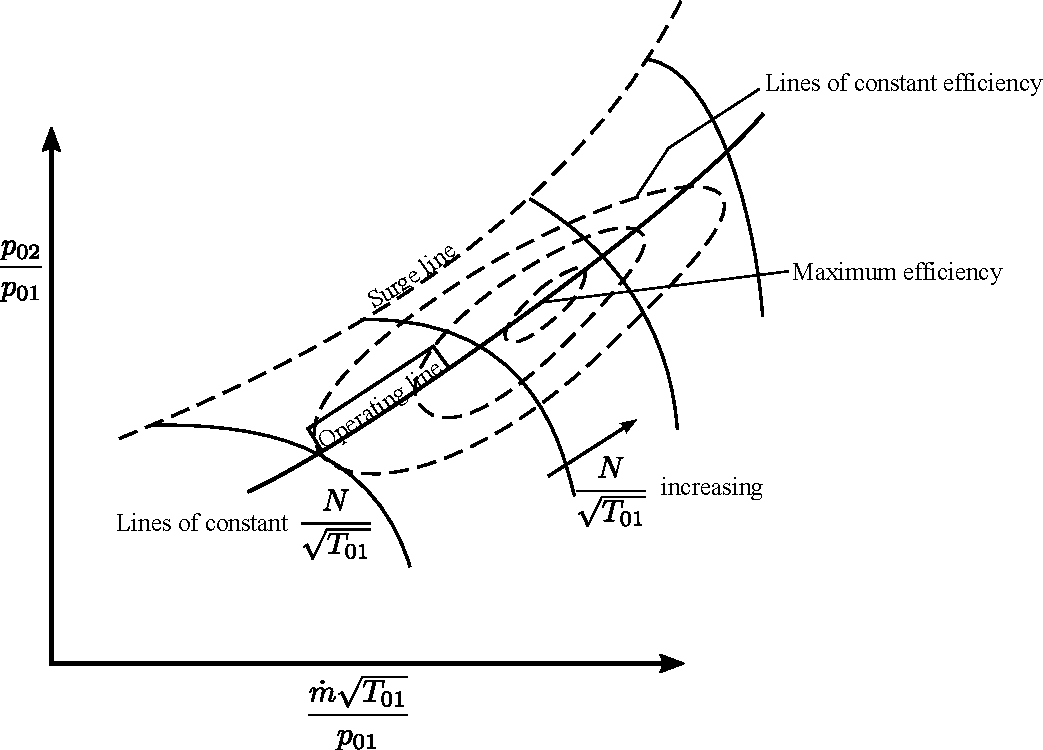
\includegraphics[width=.8\textwidth]{fig/secondo_8.pdf}
\caption{}
\label{fig:secondo_8}
\end{figure}
Guardando ai diagrammi si vede che abbiamo un fenomeno noto come ingolfamento del compressore. Intendiamo il raggiungimento di quella condizione di funzionamento in cui non è più possibile variare la portata variando il rapporto delle pressioni attorno alla macchina.
Questo perchè in qualche punto si raggiungono le condizioni di flusso sonico e quindi, ricordando lo studio dell’ugello convergente-divergente, abbiamo un
blocco sonico delle portata.

\section{Richiamo di termodinamica}
Lo scambio termico è trascurabile per i bassi tempi di residenza del fluido nel condotto.

Rotore adiabatico
\begin{equation}
L_{12}^{'} = h_{t1}-h_{t2}
\end{equation}
\begin{equation}
h_t=h+\frac{c^2}{2}+gz
\end{equation}
\begin{equation}
L_{12}^{'} = \begin{cases} u_1 c_{u1}-u_2 c_{u2}\\
\cfrac{c_1^2-c_2^2}{2}+\cfrac{u_1^2-u_2^2}{2}-\cfrac{w_1^2-w^2}{2} \end{cases}
\end{equation}

Naturalmente il lavoro è stato scritto, in base alle note convenzioni, per una macchina motrice.

Il lavoro è composto da una parte cinetica ($c$) e da una parte statica ($u,w$). 

Risulta chiaro che una macchina radiale avrà anche le componenti statiche, a differenza di una macchina puramente assiale, potra quindi, a parità di stadi, eseguire un maggior lavoro.

Ponendomi come osservatore relativo rispetto al rotore posso scrivere
\begin{equation}
u_1 c_{u1} - u_2 c_{u2} = h_1 + \frac{c_1^2}{2}+gz_1-h_2-\frac{c_2^2}{2}-gz_2
\end{equation}
Posso quindi definire la rotalpia come grandezza di stato:
\begin{equation}
h+\frac{c^2}{2}+gz-u c_u = cost. = I
\end{equation}

Riassumento:
\begin{itemize}
\item $I=cost.$ in un rotore adiabatico;
\item $h_t=cost.$ in uno statore adiabatico.
\end{itemize}

Posso esprimere tutte le grandezze fin'ora viste in un piano $T-s$ o $h-s$.

I rendimenti sono da sbobinare.
\pagebreak